\section{Měření polohy - principy odporové, indukčnostní, kapacitní}
\subsection{Odporové snímače polohy}

\subsubsection{Snímače se skokovou změnou odporu}
Mechanicky ovládané kontakty:
\begin{itemize}
    \item Mechanické mikrospínače - ovládání světla
    \item Parametry: Rozsahy síly potřebné pro spínání, velikost proudu/napětí které mohou spínat(větší problém s DC proudy), životnost z pohledu počtu spínání(rychlost mechanické únavy, klasicky \(10^6\) sepnutí)
\end{itemize}
Magneticky ovládané kontakty:
\begin{itemize}
    \item Jazýčková relé - kontakty z magneticky měkkého materiálu ovládané polem permamentního magnetu
    \item Princip - k relé přibližujeme magnet, přiblížením vzniká přitažlivá síla mezi kontakty relé
    \item Parametry - spínané proudy(jednotky mA), max počet přepnutí
    \item Kontakty se mohou slepit kvůli přiliš silné magnetizaci
    \item Měření rychlosti na kole, otevření zavření dveří, atd...
\end{itemize}
\begin{figure}[h!]
    \centering
    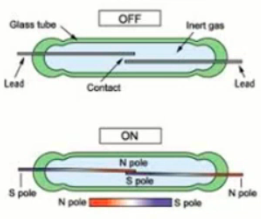
\includegraphics[scale = 0.5]{img/JazRele.png}
\end{figure}
\subsubsection{Snímače s plynulou změnou odporu}
Odporové potenciometry s pohyblivým kontaktem mechanicky spojeným s měřenou veličinou.\\
Na nevodivé podložce je nanesena vodivá vrstva, přes kterou přejíždí pohyblivý kontakt a měříme odpor mezi jezdcem a jedním z okraju vodivé dráhy.\\
Dělení podle typu jezdce:
\begin{itemize}
    \item Rotační jezdec - měření úhlového posunutí
    \item Přímočarý jezdec - měření polohy nebo lineárního posunutí
    \item Spirálový jezdec - helipot typicky s 10 závity, rozsah větší jak 360°
\end{itemize}
Lankem ovládané potenciometry, mají rozsah až 40m, rychlost 2m/s.
\begin{figure}[h!]
    \centering
    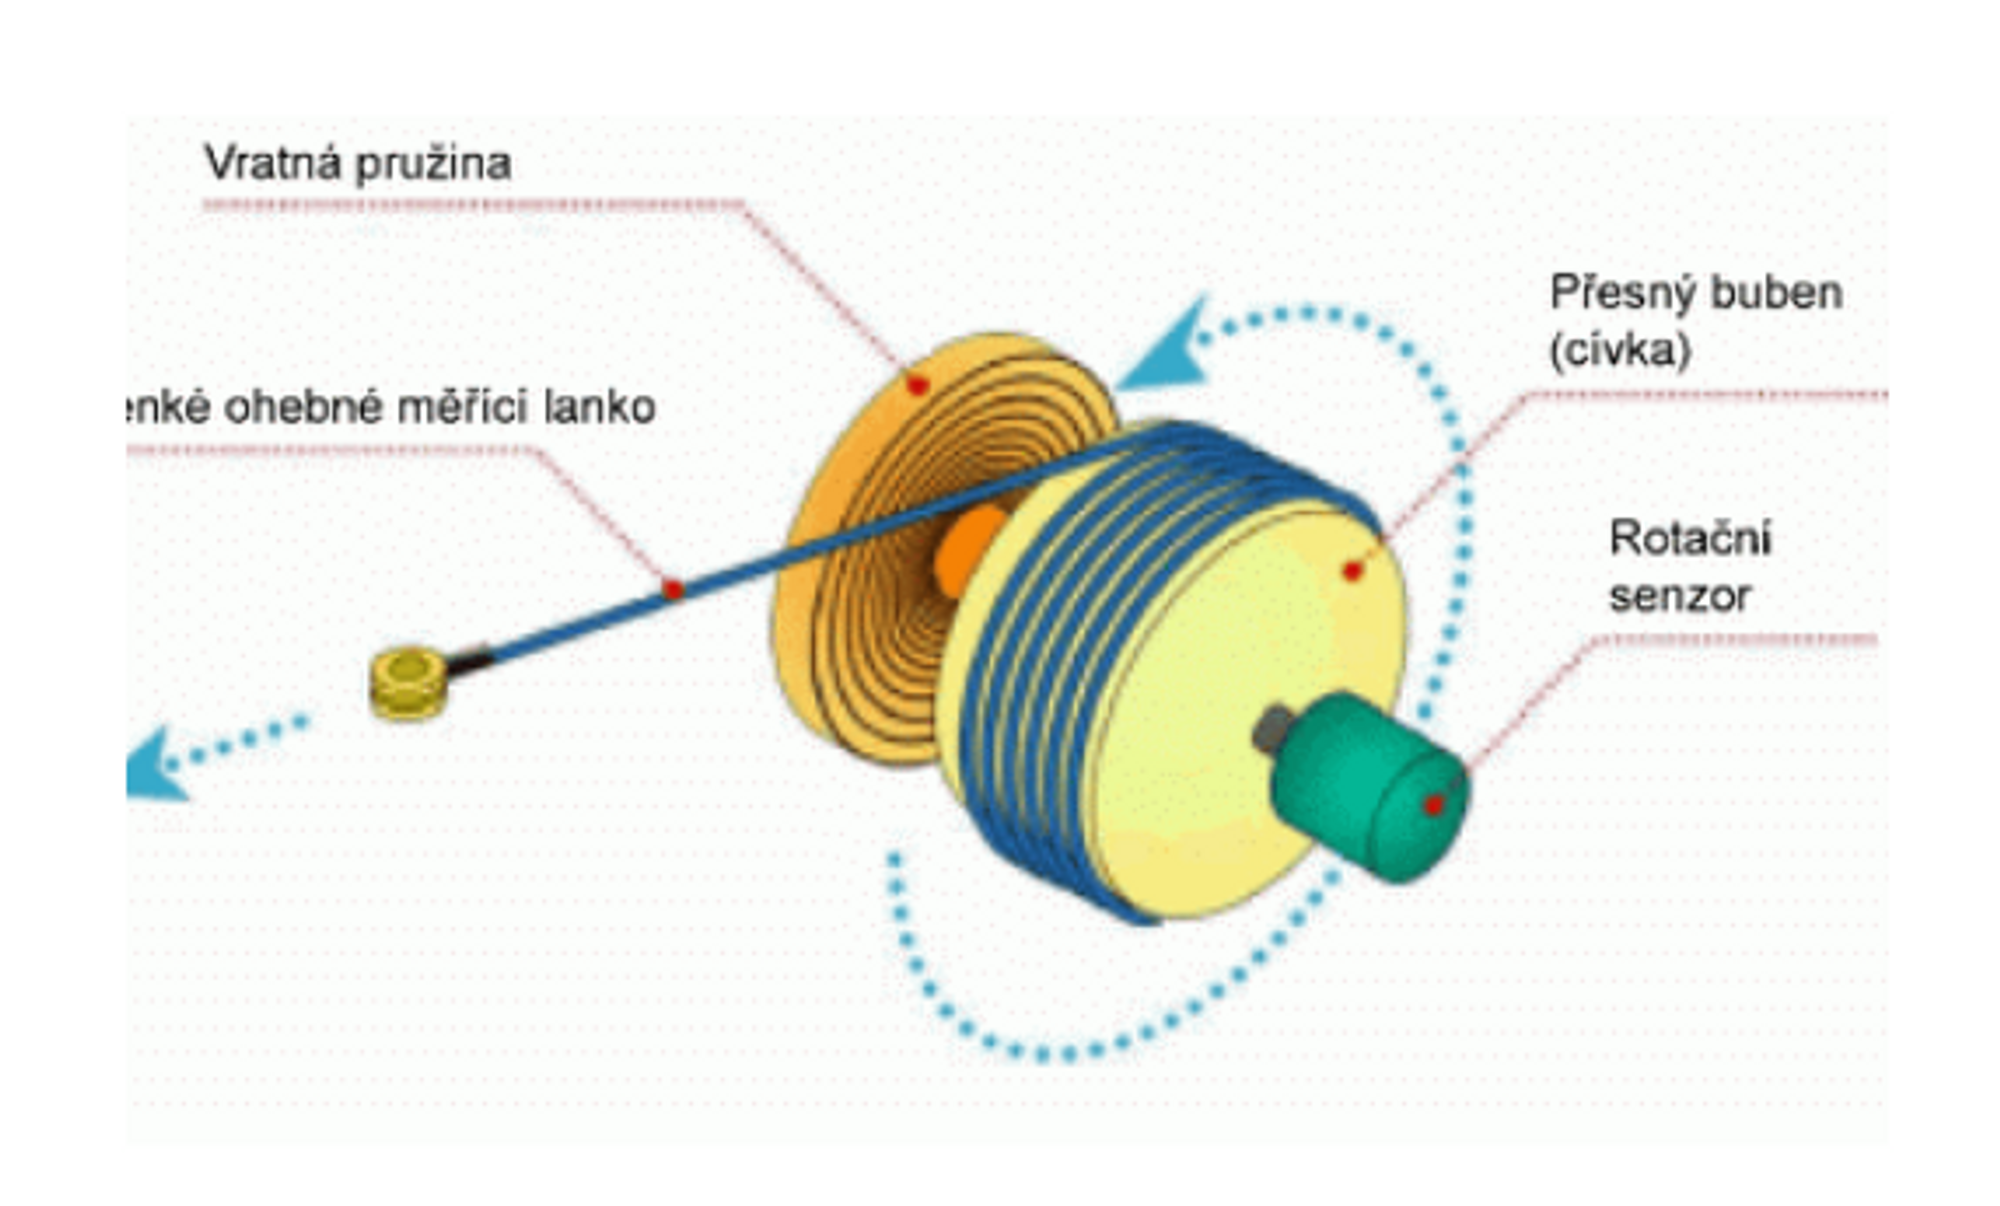
\includegraphics[scale = 0.1]{img/Lanko.png}
\end{figure}

\subsubsection{Zapojení odporových snímačů}
\begin{figure}[h!]
    \centering
    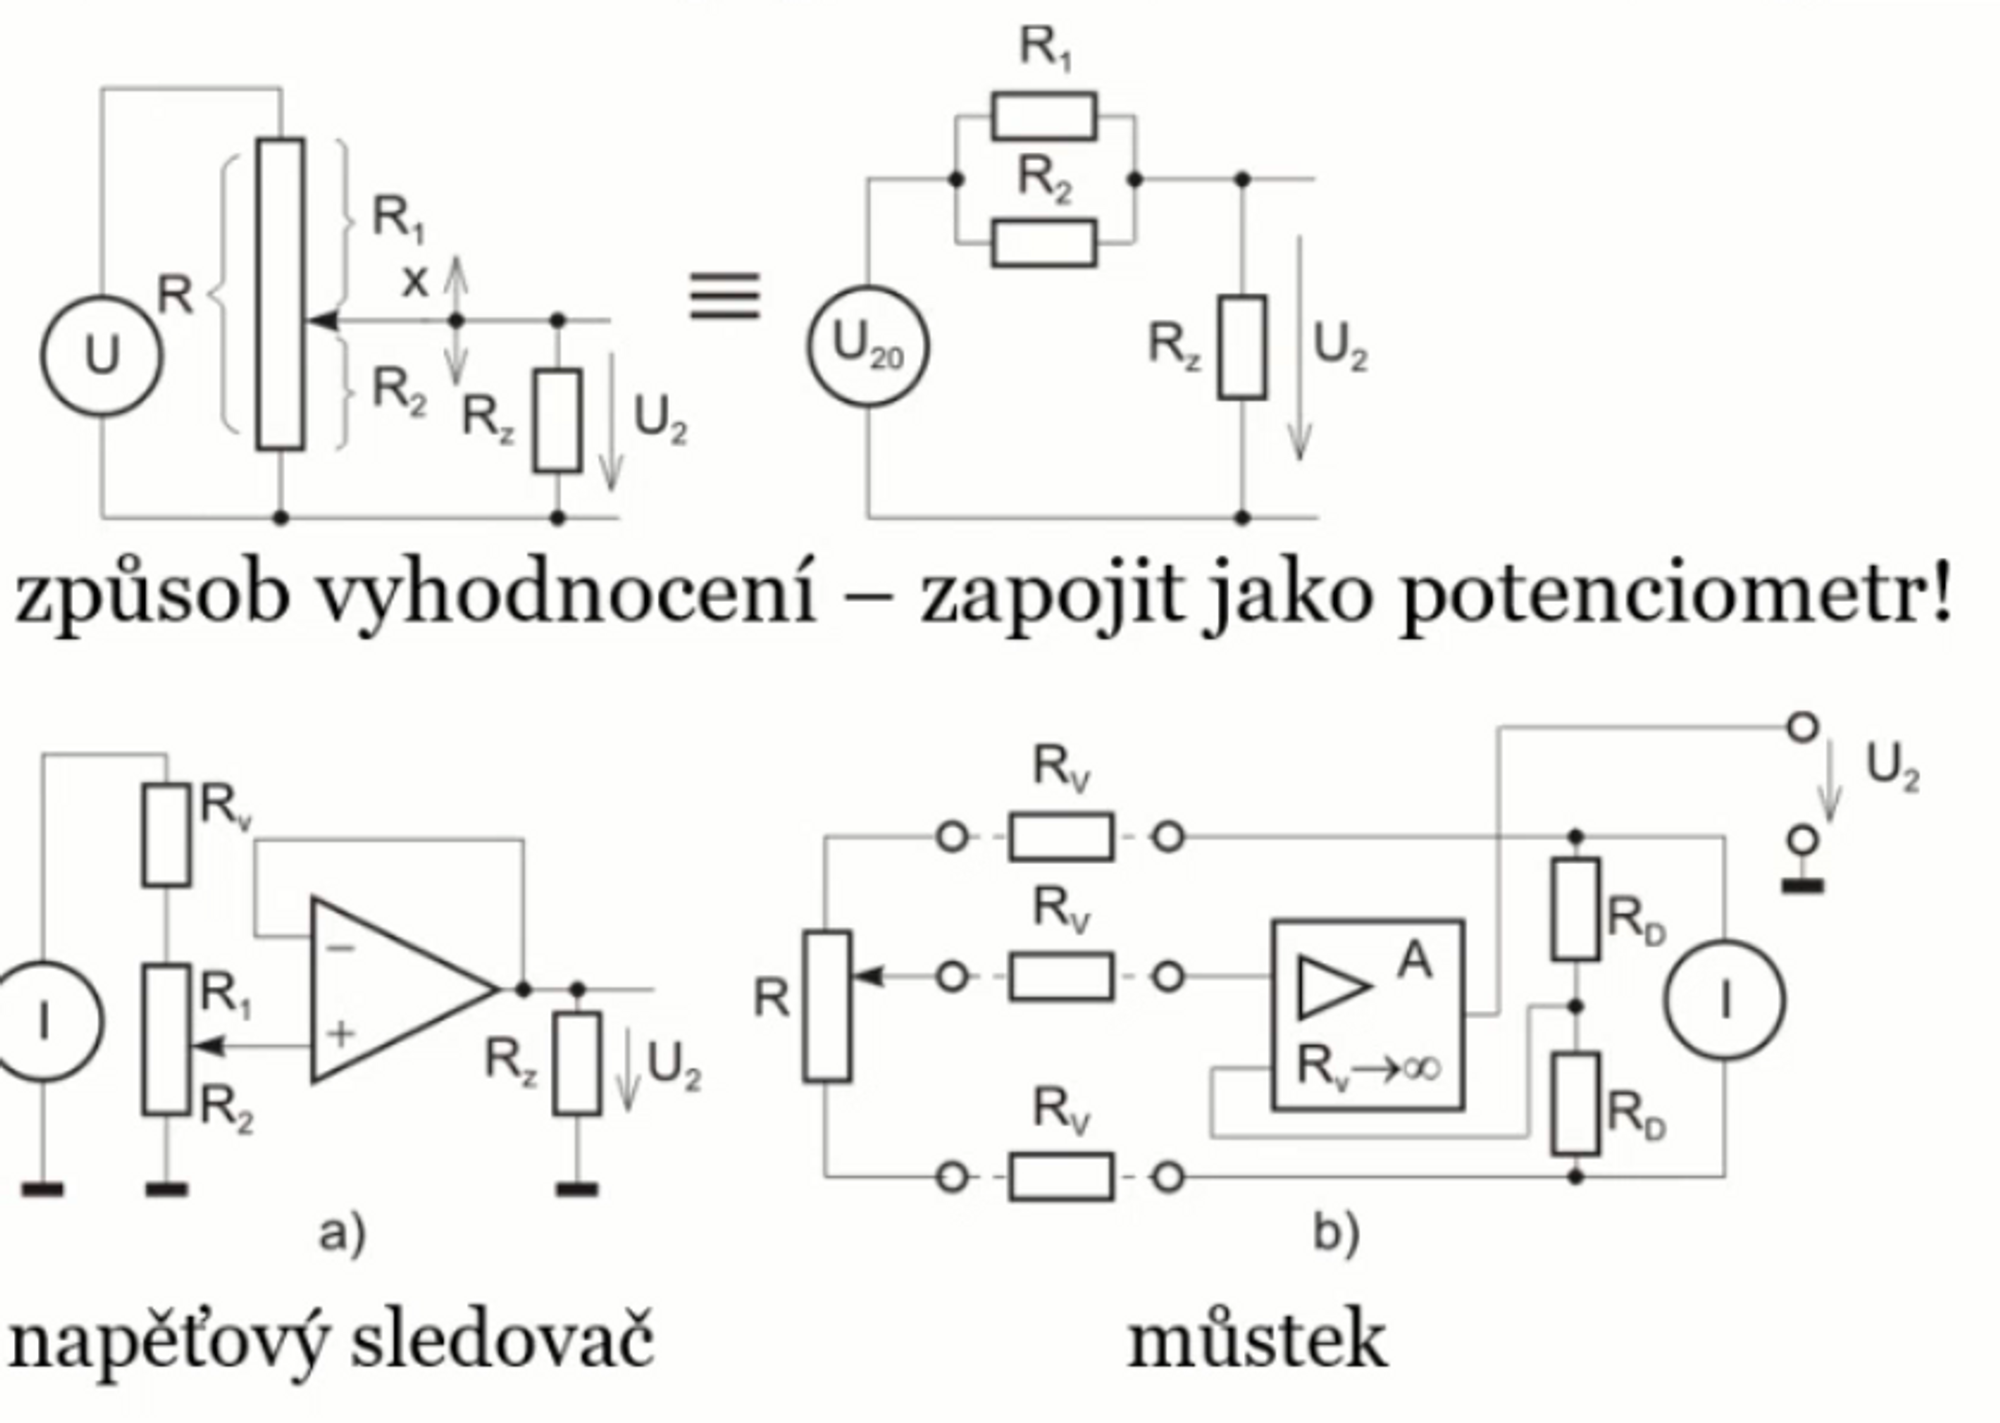
\includegraphics[scale = 0.1]{img/ZapojeniOdp.png}
\end{figure}

\subsubsection{Výhody}
\begin{itemize}
    \item jednoduché zpracování signálu
    \item reprodukovatelnost, linearita
    \item odolnost proti vibracím - ne tak uplně, jen běžné průmyslové vibrace tlumí
\end{itemize}
\subsubsection{Nevýhody}
\begin{itemize}
    \item kontaktní princip
    \item šum
    \item životnost
    \item dynamické vlastnosti
    \item omezený ztrátový výkon
\end{itemize}

\section{Měření polohy - principy optické, magnetické, ultrazvukové}


\section{Měření vibrací, rychlosti, zrychlení, akcelerometry, snímače úhlové rychlosti }


\section{Tenzometry, snímače síly, hmotnosti, momentu a tlaku }


\section{Měření průtoku, základní principy objemových, rychlostních a hmotnostních průtokoměrů}


\section{Kontaktní snímače teploty (dilatační, odporové, termoelektrické)}


\section{Měření záření (tepelné a kvantové snímače IR záření, snímače ionizujícího záření)}


\section{Chemické snímače}